\chapter{Semantics}
\label{semantics}
\section{Abstract Syntax for Ezuino}
At this stage, we got the syntax made, and we have a general idea of the language. The next step is to construct semantics for the Ezuino programming language. This chapter will go through each semantic rule, in categorized. 
Before we can start on semantics, we need a table, to provide an overview of the short names in each semantic. This can be  reviewed in figure \ref{semCat}.
\begin{figure}[H]
\centering
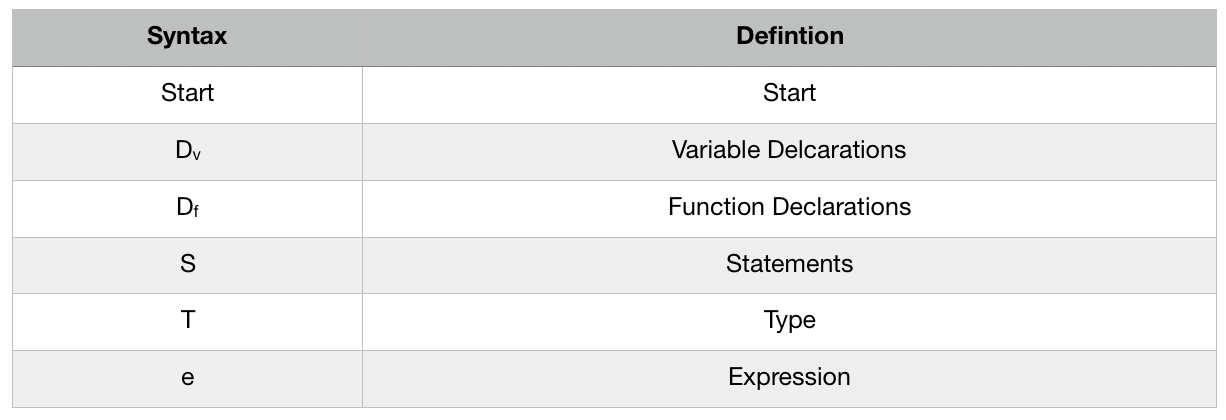
\includegraphics[scale=0.75]{figures/semantics/categories.png}
\caption{Table of Reserved Keywords}
\label{semCat}
\end{figure}


\subsection{Formation Rules}
%% SCOPE RULES INERT HERE
\section{Type System Semantics}
The Ezuino programming language data types is only primitive types. This is denoted in future references as :
\begin{table}[H]
    \centering
    \begin{longtable}[c] { r c }
      
        \( { T_{TP} = (string,\ bool,\ double,\ integer)} \) \\
    \end{longtable}
    \caption{}\label{s-empty}
\end{table}





\subsection{Type Environment}
%\begin{table}[H]
%    \begin{center}
%    \begin{longtable}[c] { r c }
%        [Example_{test}] 
%        & 
%        \( \dfrac{T E(T x; D_v, T E) = T E(D_v, T E[x 7 \mapsto T])} 
%        {T E(T x; D_v, T E) = T E(D_v, T E[x 7 \mapsto T])} \) 
%        \\ \\
%        & 
%        \( {where \ T \ \epsilon \ T_{primitive} \ \textbackslash \ %\{void,\ bool,\ text,\ number\}} \)
%    \end{longtable}
%    \caption{}\label{s-empty}
%        \end{center}
%\end{table}
Updating a type environment with empty have no effect on the type environment.
\begin{table}[H]
    \centering
    \begin{longtable}[c] { r c }
        $[Update_{empty}]$ & 
        \( {TE(\epsilon, TE) = TE} \) \\
    \end{longtable}
    \caption{}\label{s-empty}
\end{table}


Declaring a variable updates the type environment with the variables type.
\begin{table}[H]
    \begin{center}
    \begin{longtable}[c] { r c }
        $[Update_{D_v}]4$ 
        & 
        \( {T E(T \ x;\ D_v, T E) = T E(D_v,\ T E[x \mapsto T])} \) 
        \\ \\
        & 
        \( {where \ T \ \epsilon \ T_{pt}} \)
    \end{longtable}
    \caption{}\label{s-empty}
        \end{center}
\end{table}

Declaring a function updates the type environment with the functions formal parameters and return type.
\begin{table}[H]
    \begin{center}
    \begin{longtable}[c] { r c }
        $[Update_{D_f}]$ 
        & 
        \( T E(T \ f(T_1 x_1,\ ...,\ T_k x_k)S \ D_f
,\ T E) = T E(D_f
,\ T E[f  \mapsto  (T_1,\ ...\, T_n \ × \ T_r)])
( \) 
    \end{longtable}
    \caption{}\label{s-empty}
        \end{center}
\end{table}

\subsubsection*{Expressions}
Expressions are the core of most programming operations. Ezuino supports parenthesis, arithmetic and logical expressions. Since casting is explicit integers and doubles are not compatible and their type rules are therefore separated despite both using type rules operating on numbers. As it was argued in \ref{language-features} string also supports the equality and concatenation operation as these are seen as essential features of strings.
\begin{table}[H]
    \begin{center}
    \begin{longtable}[c] { r c }
        $[Parenthesis] $
        & 
        \( \dfrac{T E  \vdash  e  :  T}{T E  \vdash  (e)  :  T} \) 
        \\ \\
        & 
        \( {where \ T \ \epsilon \ \{ bool,\ string,\ int,\ double\}} \)
    \end{longtable}
    \caption{}\label{s-empty}
        \end{center}
\end{table}
 
\begin{table}[H]
    \begin{center}
    \begin{longtable}[c] { r c }
        $[ArithInt_{e}]$ 
        & 
        \( \dfrac{TE \vdash e_{1} :  int \ \ TE \vdash e_{2} : int} 
        {\ TE \vdash e_{1} \ op \ e_{2} : int} \) 
        \\ \\
        & 
        \( {where \ op \ \epsilon \ \{+, \ -, \ /, \ *\} } \)
    \end{longtable}
    \caption{}\label{s-empty}
        \end{center}
\end{table}
\begin{table}[H]
    \begin{center}
    \begin{longtable}[c] { r c }
        $[ArithDouble_{e}]$ 
        & 
        \( \dfrac{TE \vdash e_{1} : double \ \ TE \vdash e_{2} :  double} 
        {\ TE \vdash e_{1} \ op \ e_{2} : double} \) 
        \\ \\
        & 
        \( {where \ op \ \epsilon \ \{+, \ -, \ /, \ *\} } \)
    \end{longtable}
    \caption{}\label{s-empty}
        \end{center}
\end{table}
\begin{table}[H]
    \begin{center}
    \begin{longtable}[c] { r c }
        $[IntRelation_{e}]$ 
        & 
        \( \dfrac{T E  \vdash  e_1  :  int \ T E  \vdash  e_2  :  int}{T E  \vdash  e_1 \ op \ e_2  :  bool} \) 
        \\ \\
        & 
        \( {where \ op \ \epsilon \ \{<,\ >,\ <=,\ >=,\ =,\ !=\}} \)
    \end{longtable}
    \caption{}\label{s-empty}
        \end{center}
\end{table}

\begin{table}[H]
    \begin{center}
    \begin{longtable}[c] { r c }
        $[DoubleRelation_{e}]$ 
        & 
        \( \dfrac{T E  \vdash  e_1  : double \ T E  \vdash  e_2  :  double}{T E  \vdash  e_1 \ op \ e_2  :  bool} \) 
        \\ \\
        & 
        \( {where \ op \ \epsilon \ \{<,\ >,\ <=,\ >=,\ =,\ !=\}} \)
    \end{longtable}
    \caption{}\label{s-empty}
        \end{center}
\end{table}
\begin{table}[H]
    \begin{center}
    \begin{longtable}[c] { r c }
        $[StringRelation_{e}]$ 
        & 
        \( \dfrac{T E  \vdash  e_1  :  string \ TE  \vdash  e_2  :  string }{TE  \vdash  e_1 \ op \ e_2  :  bool} \) 
        \\ \\
        & 
        \( {where \ op \ \epsilon \ \{=, \ !=\}} \)
    \end{longtable}
    \caption{}\label{s-empty}
        \end{center}
\end{table}


\begin{table}[H]
    \begin{center}
    \begin{longtable}[c] { r c }
        $[Logical_{e}]$ 
        & 
        \( \dfrac{T E  \vdash  e_1  :  string \ TE  \vdash  e_2  :  string }{T E  \vdash  e_1 \ op \ e_2  :  bool} \) 
        \\ \\
        & 
        \( {where \ op \ \epsilon \ \{=,\ !=\, AND,\ OR,\ !,\ <,\ <=,\ >,\ >= \}} \)
    \end{longtable}
    \caption{}\label{s-empty}
        \end{center}
\end{table}

\begin{table}[H]
    \begin{center}
    \begin{longtable}[c] { r c }
        $[Concat]$ 
        & 
        \( \dfrac{TE \vdash  e_1  :  string \ \ TE  \vdash  e_2  :  string }{TE \vdash  e_1 \ op \ e_2  :  string} \) 
                 \\ \\
        & 
        \( {where \ op \ \epsilon \ \{+ \}} \)
    \end{longtable}
    \caption{}\label{s-empty}
        \end{center}
\end{table}

\begin{table}[H]
    \begin{center}
    \begin{longtable}[c] { r c }
        $[NegInt_{e}]$ 
        & 
        \( \dfrac{T E  \vdash  e_1  :  int}{T E  \vdash  -e_1  :  int} \) 
    \end{longtable}
    \caption{}\label{s-empty}
        \end{center}
\end{table}

\begin{table}[H]
    \begin{center}
    \begin{longtable}[c] { r c }
        $[NegDouble_{e}]$ 
        & 
        \( \dfrac{T E  \vdash  e_1  :  double}{T E  \vdash  -e_1  :  double} \) 
    \end{longtable}
    \caption{}\label{s-empty}
        \end{center}
\end{table}

\begin{table}[H]
    \begin{center}
    \begin{longtable}[c] { r c }
        $[Not_{e}]$ 
        & 
        \( \dfrac{T E  \vdash  e_1  :  bool}{T E  \vdash  !e_1  :  bool} \) 
    \end{longtable}
    \caption{}\label{s-empty}
        \end{center}
\end{table}

\begin{table}[H]
    \begin{center}
    \begin{longtable}[c] { r c }
        $[Var]$ 
        & 
        \( {T E  \vdash x  :  T} {where \ T E(x)=\ T} \)
         \\ \\
        & 
        \( {and \ T \ \epsilon \ \{bool,\ string,\ int,\ double\}} \)
    \end{longtable}
    \caption{}\label{s-empty}
        \end{center}
\end{table}
In a function declaration the return type is specified and the types for the formal parameters are saved in the type environment. Afterwards there can be statements and other function declarations. \\
Every statement in the function declaration must be OK in regards to the declared return type. This means that return statements in if and else statements as well as return statements in the function declaration body must return the declared return type. \\ 
Functions declared in a function declaration must be well typed as well.
\begin{table}[H]
    \begin{center}
    \begin{longtable}[c] { r c }
        $[FuncDcl]$ 
        & 
        \( \dfrac{TE' \vdash S : OK \ \ TE \vdash D_{f}: OK} 
        {T E \vdash T_r \ f(T_1 \ x_1,\ ...,\ T_n,\ x_n)S D_f : OK} \) 
        \\ \\
        & 
        \( {where \ TE' = TE[r \mapsto T_r]} \)
    \end{longtable}
    \caption{}\label{s-empty}
        \end{center}
\end{table}

In a while loop the expression must be a bool type while the statement inside the the while loop must be OK.
\begin{table}[H]
    \begin{center}
    \begin{longtable}[c] { r c }
        $[While]$ 
        & 
        \( \dfrac{T E  \vdash e  :  bool \ T E \vdash S : OK}{T E \vdash while(e) \ S : OK} \)

    \end{longtable}
    \caption{}\label{s-empty}
        \end{center}
\end{table}

Check if and else expression are OK, and if they are OK then also make sure the statements of the if and else statements are OK.
\begin{table}[H]
    \begin{center}
    \begin{longtable}[c] { r c }
        $[If - else]$ 
        & 
        \( \dfrac{T E  \vdash e  :  bool \ T E \vdash S_1 : OK \ OK \ T E \vdash S_2 : OK}
        {T E \vdash if(e) \ S_1 \ else \ S_2 : OK} \)

    \end{longtable}
    \caption{}\label{s-empty}
        \end{center}
\end{table}

The return statement is only correct when its expression type is the same as the function type. The function return type is found in the type environment
\begin{table}[H]
    \begin{center}
    \begin{longtable}[c] { r c }
        $[Return]$ 
        & 
        \( \dfrac{T E  \vdash e  :  T}{T E \vdash return \ e : OK} \)
         \\ \\
        & 
        \( {if \ TE(r) = T } \)

    \end{longtable}
    \caption{}\label{s-empty}
        \end{center}
\end{table}








\subsection{Blocks}
Blocks can be referred to as the body of if-else statenents, while statements and functions. Each block has a specific scoping, which is handled by the Symbol Table as described in \ref{Block_Structure_Symbol_Tables}. The first symbol table will start with a global scope and add a scope for each new block that is being created. In table \ref{block}, we can see that we can look back to the previously known variable declarations.
\begin{table}[H]
    \begin{center}
    \begin{longtable}[c] { r c }
        $[Block]$ 
        & 
        \( \dfrac{TE' \vdash S : OK} 
        {TE \vdash D_v S : OK} \) 
        \\ \\
        & 
        \( {where \ TE' = TE(D_v, TE)} \)
    \end{longtable}
    \caption{}\label{block}
        \end{center}
\end{table}

Table \ref{active-block} is the active block which is the block we’re currently in. Unlike table \ref{block}, it cannot know its previous blocks, however, it is the one which are current for each block.
\begin{table}[H]
    \begin{center}
    \begin{longtable}[c] { r c }
        $[Block_{current}]$ 
        & 
        \( \dfrac{TE \vdash D_{v} : OK \ TE \vdash S : OK} 
        {TE \vdash current \ D_{v} \ S \ end  :  OK} \)
    \end{longtable}
    \caption{}\label{active-block}
        \end{center}
\end{table}

\section{Structural Operation Semantics}
\subsection{Environment-Store Model}
